% 图 77.5 —— 由 `checks/emit_hand.py` 自动拼出（probe 精测 + prims2 图元分解）
%%
% ⚠ 这是**稿子不是成品**：跑 `checks/checkhand.py 77.5` 看指标 + 看叠合图。
%%
%% ⚠ 待核：
%   · 本图 probe 报出阴影族 2 个 —— **本脚本不生成阴影**（要照原书手写）；prims2 的 strokes 里可能含阴影线，核对时留意别画重
%   · 可疑字形 2 项（空心圈 ⊙ 常被认成字母 o）—— 见文件末
%%
\documentclass[12pt]{standalone}
\usepackage{fontspec}
\setsansfont{Arial}
\newfontfamily\mfallback{DejaVu Sans}
\usepackage{tikz}
\begin{document}
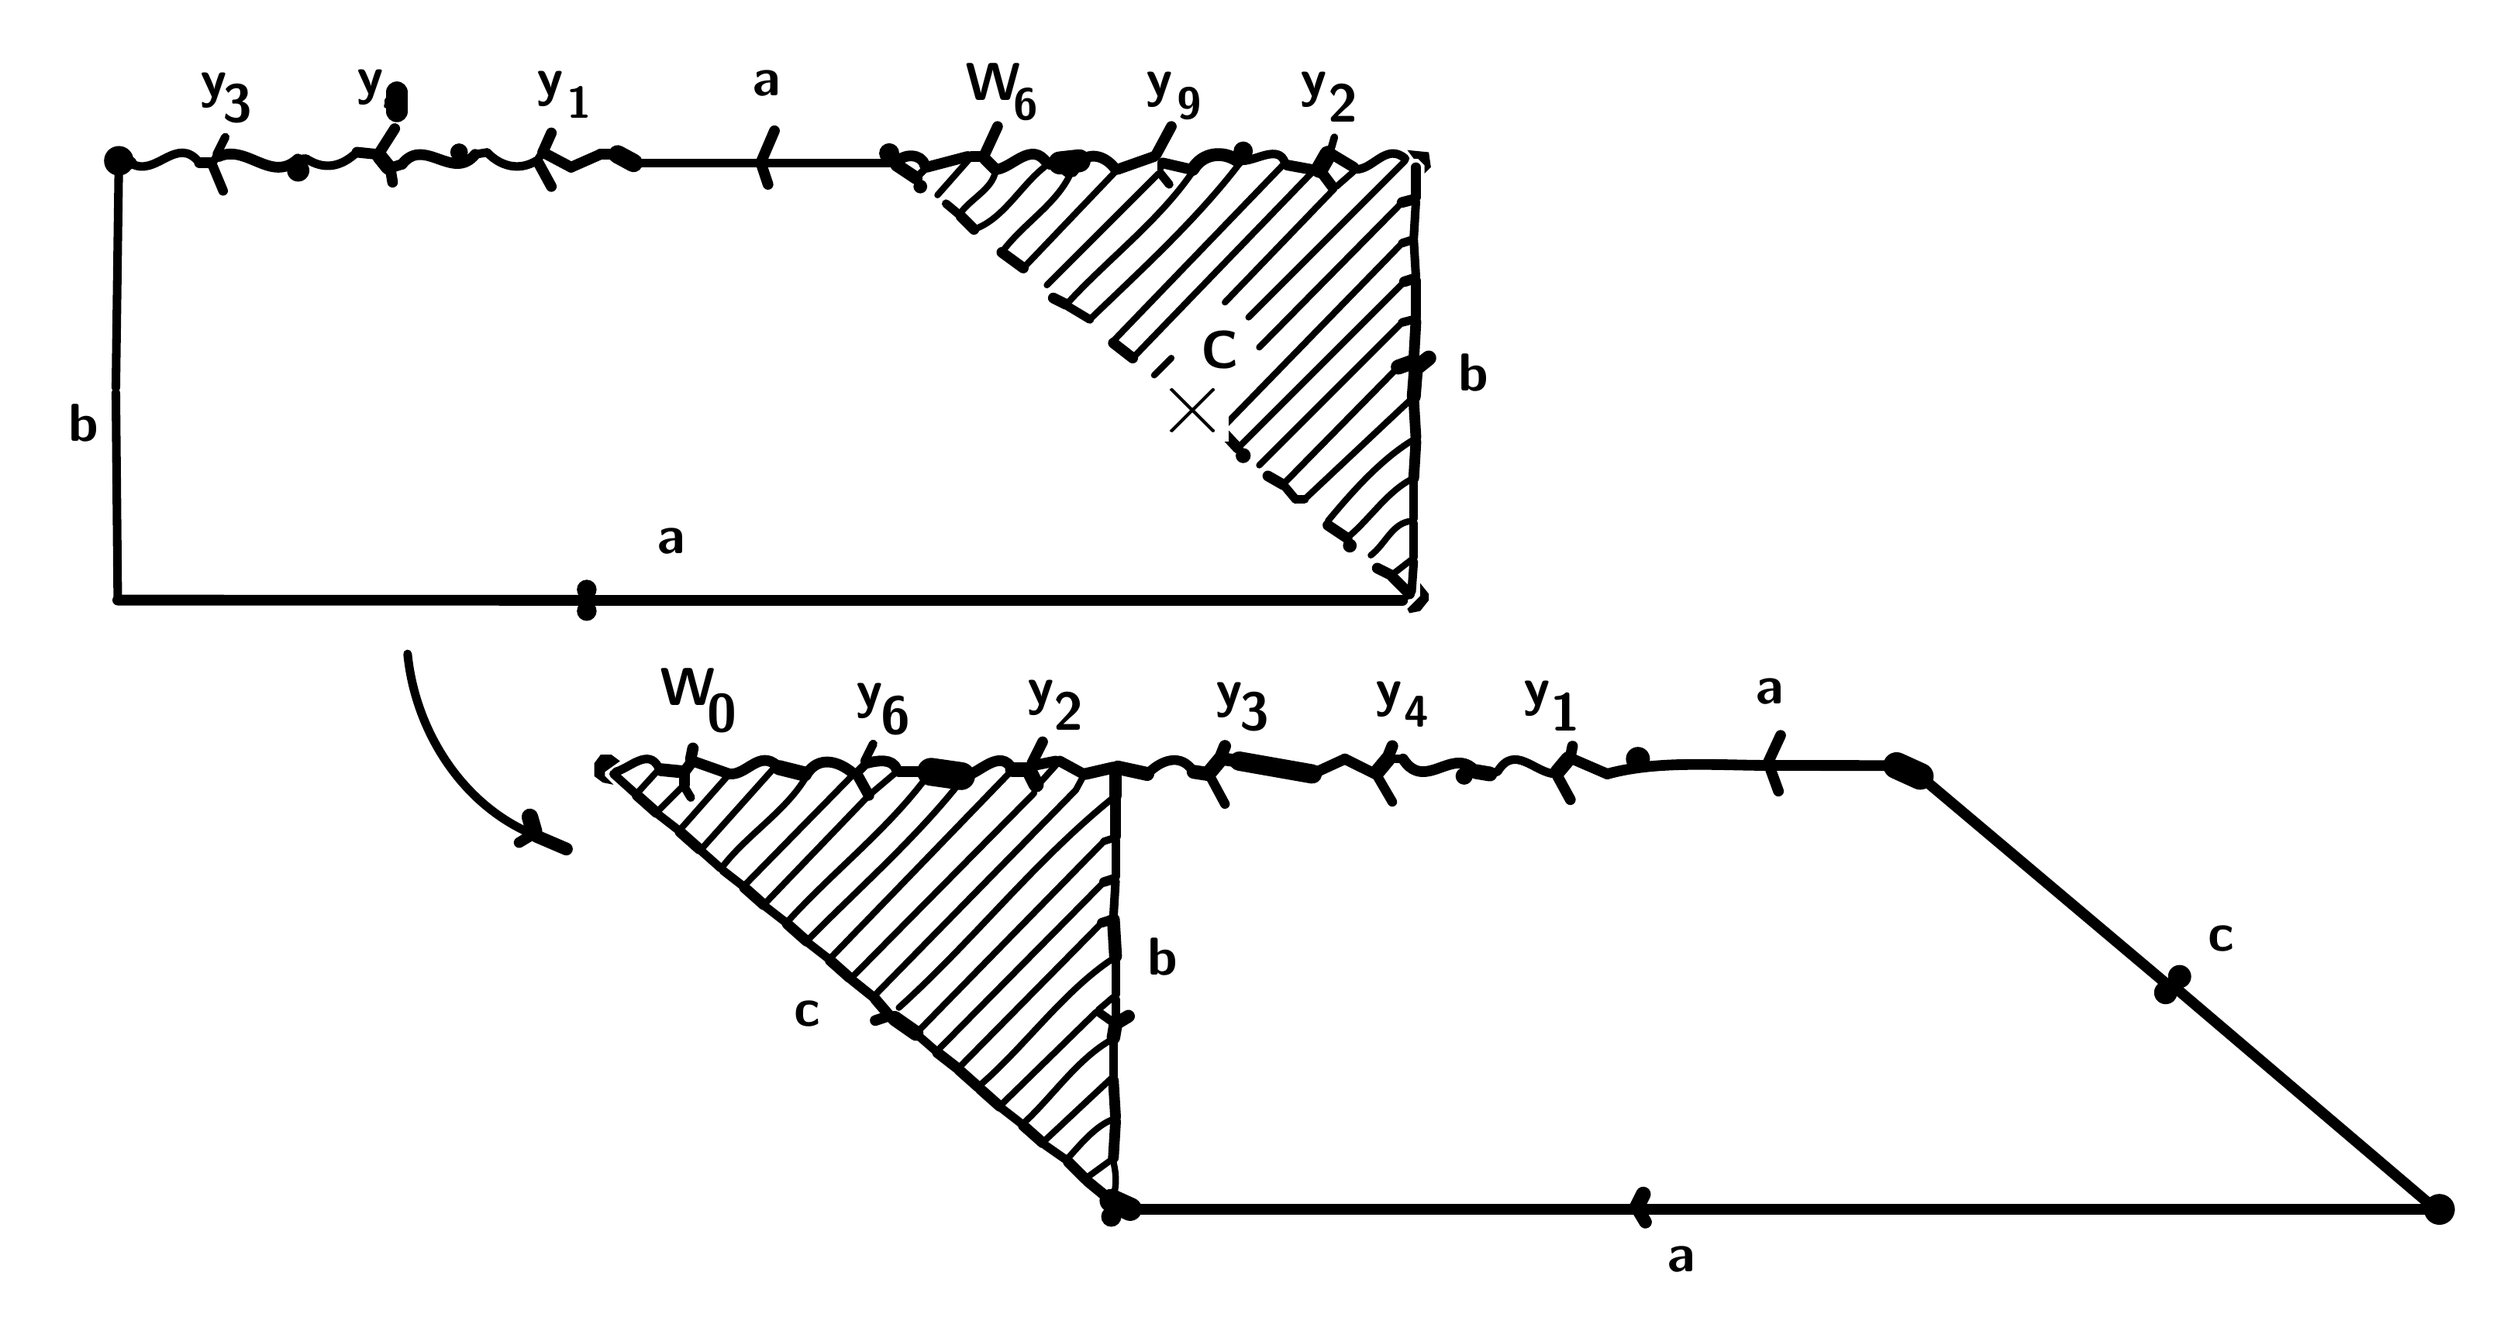
\begin{tikzpicture}[x=1pt, y=-1pt, line width=6.3pt, line cap=round, line join=round]

  %% ════ 填充区（prims2 的 fills）════
  \fill (174.0,29.0) -- (169.0,37.0) -- (169.0,40.0) -- (176.0,44.0) -- (178.0,42.0) -- (178.0,30.0) -- cycle;
  \fill (646.0,60.0) -- (649.0,64.0) -- (651.0,64.0) -- (654.0,67.0) -- (654.0,71.0) -- (657.0,68.0) -- (656.0,61.0) -- cycle;
  \fill (652.0,262.0) -- (652.0,268.0) -- (646.0,274.0) -- (647.0,276.0) -- (652.0,275.0) -- (656.0,270.0) -- (656.0,267.0) -- cycle;
  \fill (270.0,342.0) -- (267.0,346.0) -- (267.0,352.0) -- (271.0,355.0) -- (276.0,356.0) -- (272.0,352.0) -- (272.0,350.0) -- (279.0,345.0) -- (275.0,342.0) -- cycle;

  %% ════ 直线段（prims2 的 strokes）════
  \draw[line width=6.3pt] (510.0,468.0) -- (509.0,474.0);
  \draw[line width=5.0pt] (443.0,63.0) -- (448.0,63.0);
  \draw[line width=7.1pt] (1126.0,556.0) -- (1123.0,552.0);
  \draw[line width=5.0pt] (722.0,363.0) -- (716.0,352.0);
  \draw[line width=5.0pt] (330.0,351.0) -- (313.0,345.0);
  \draw[line width=3.0pt] (330.0,351.0) -- (307.0,377.0);
  \draw[line width=5.0pt] (265.0,270.0) -- (643.8,270.0);
  \draw[line width=3.0pt] (643.8,270.0) -- (646.0,268.0);
  \draw[line width=4.5pt] (554.0,352.0) -- (561.0,365.0);
  \draw[line width=3.0pt] (477.0,522.0) -- (508.0,493.0);
  \draw[line width=5.0pt] (472.0,347.0) -- (482.0,345.0);
  \draw[line width=5.0pt] (611.0,77.0) -- (605.0,69.0);
  \draw[line width=3.0pt] (577.0,207.0) -- (643.6,140.4);
  \draw[line width=4.0pt] (643.6,140.4) -- (649.0,139.0);
  \draw[line width=10.7pt] (493.0,65.0) -- (484.0,66.0);
  \draw[line width=4.0pt] (437.0,90.0) -- (431.0,85.0);
  \draw[line width=5.0pt] (309.0,356.0) -- (309.0,351.0);
  \draw[line width=3.8pt] (89.0,66.0) -- (91.0,63.0);
  \draw[line width=4.0pt] (649.0,102.0) -- (650.0,119.0);
  \draw[line width=5.0pt] (247.0,77.0) -- (241.0,66.0);
  \draw[line width=4.0pt] (44.0,173.0) -- (44.9,269.9);
  \draw[line width=5.0pt] (44.9,269.9) -- (263.0,270.0);
  \draw[line width=3.0pt] (297.0,349.0) -- (287.0,360.0);
  \draw[line width=4.0pt] (509.0,467.0) -- (502.0,462.0);
  \draw[line width=5.0pt] (1123.0,552.0) -- (1002.0,449.0);
  \draw[line width=3.0pt] (1123.0,552.0) -- (1120.8,554.0);
  \draw[line width=5.0pt] (1120.8,554.0) -- (755.0,554.0);
  \draw[line width=5.0pt] (404.0,463.0) -- (398.0,456.0);
  \draw[line width=4.0pt] (509.0,418.0) -- (510.0,401.0);
  \draw[line width=7.0pt] (721.0,344.0) -- (716.0,350.0);
  \draw[line width=3.0pt] (497.0,539.0) -- (508.0,531.0);
  \draw[line width=5.3pt] (312.0,344.0) -- (313.0,339.0);
  \draw[line width=7.0pt] (559.0,344.0) -- (554.0,350.0);
  \draw[line width=3.0pt] (297.0,368.0) -- (308.0,357.0);
  \draw[line width=4.0pt] (393.0,345.0) -- (397.0,337.0);
  \draw[line width=5.0pt] (649.0,83.0) -- (643.6,84.4);
  \draw[line width=3.0pt] (643.6,84.4) -- (577.0,152.0);
  \draw[line width=5.0pt] (243.0,61.0) -- (247.0,52.0);
  \draw[line width=3.8pt] (243.0,61.0) -- (241.0,64.0);
  \draw[line width=5.0pt] (243.0,61.0) -- (256.2,68.0);
  \draw[line width=5.0pt] (256.2,68.0) -- (269.8,62.0);
  \draw[line width=5.0pt] (269.8,62.0) -- (277.9,62.0);
  \draw[line width=8.6pt] (277.9,62.0) -- (285.3,66.0);
  \draw[line width=4.0pt] (285.3,66.0) -- (344.0,66.0);
  \draw[line width=4.0pt] (488.0,133.0) -- (498.0,139.0);
  \draw[line width=4.0pt] (650.0,84.0) -- (649.0,101.0);
  \draw[line width=4.0pt] (531.0,71.0) -- (535.0,76.0);
  \draw[line width=6.0pt] (408.0,67.0) -- (417.0,73.0);
  \draw[line width=4.0pt] (327.0,396.0) -- (336.0,403.0);
  \draw[line width=3.0pt] (645.0,65.0) -- (572.0,138.0);
  \draw[line width=4.0pt] (91.0,62.0) -- (95.0,54.0);
  \draw[line width=4.5pt] (650.0,68.0) -- (650.0,82.0);
  \draw[line width=3.0pt] (437.0,488.0) -- (503.6,420.4);
  \draw[line width=4.5pt] (503.6,420.4) -- (508.0,419.0);
  \draw[line width=4.5pt] (639.0,364.0) -- (632.0,352.0);
  \draw[line width=3.9pt] (688.1,349.9) -- (684.5,351.0);
  \draw[line width=6.9pt] (684.5,351.0) -- (677.9,349.9);
  \draw[line width=4.0pt] (644.0,344.0) -- (638.0,344.0);
  \draw[line width=4.0pt] (648.0,102.0) -- (643.6,103.4);
  \draw[line width=3.0pt] (643.6,103.4) -- (559.0,190.4);
  \draw[line width=5.0pt] (559.0,190.4) -- (567.0,199.0);
  \draw[line width=5.0pt] (348.0,76.0) -- (345.0,67.0);
  \draw[line width=5.0pt] (488.0,532.0) -- (496.0,540.0);
  \draw[line width=3.0pt] (398.0,454.0) -- (491.5,358.5);
  \draw[line width=3.0pt] (491.5,358.5) -- (495.0,352.0);
  \draw[line width=7.0pt] (648.0,159.0) -- (641.8,161.2);
  \draw[line width=3.0pt] (641.8,161.2) -- (589.0,215.0);
  \draw[line width=3.0pt] (347.0,411.0) -- (395.0,361.0);
  \draw[line width=4.0pt] (589.0,217.0) -- (594.0,223.0);
  \draw[line width=4.0pt] (594.0,223.0) -- (598.0,223.0);
  \draw[line width=3.0pt] (598.0,223.0) -- (648.0,176.0);
  \draw[line width=3.0pt] (483.0,346.0) -- (474.0,356.0);
  \draw[line width=5.0pt] (601.0,69.0) -- (590.0,67.0);
  \draw[line width=4.0pt] (217.1,61.1) -- (211.5,62.0);
  \draw[line width=4.9pt] (177.4,66.6) -- (173.0,68.0);
  \draw[line width=5.0pt] (481.0,129.0) -- (487.0,132.0);
  \draw[line width=7.0pt] (756.0,547.0) -- (753.0,553.0);
  \draw[line width=4.0pt] (649.0,250.0) -- (649.0,234.0);
  \draw[line width=5.2pt] (309.0,350.0) -- (312.0,346.0);
  \draw[line width=3.0pt] (377.0,437.0) -- (462.0,349.0);
  \draw[line width=3.0pt] (528.0,165.0) -- (536.0,157.0);
  \draw[line width=3.0pt] (530.0,71.0) -- (478.0,123.0);
  \draw[line width=5.0pt] (390.0,352.0) -- (395.0,361.0);
  \draw[line width=8.0pt] (605.0,69.0) -- (609.0,62.0);
  \draw[line width=5.0pt] (174.0,50.0) -- (167.0,61.0);
  \draw[line width=3.0pt] (639.0,258.0) -- (648.0,251.0);
  \draw[line width=3.5pt] (610.0,61.0) -- (612.0,54.0);
  \draw[line width=5.0pt] (436.0,488.0) -- (427.0,481.0);
  \draw[line width=5.0pt] (166.0,62.0) -- (156.4,61.0);
  \draw[line width=4.0pt] (132.7,64.0) -- (128.8,64.2);
  \draw[line width=5.0pt] (449.0,62.0) -- (455.0,49.0);
  \draw[line width=6.0pt] (510.0,436.0) -- (509.0,419.0);
  \draw[line width=4.0pt] (509.0,492.0) -- (509.0,475.0);
  \draw[line width=3.0pt] (468.0,114.0) -- (510.0,70.0);
  \draw[line width=5.0pt] (398.0,466.0) -- (404.0,464.0);
  \draw[line width=7.7pt] (237.0,371.0) -- (239.0,378.0);
  \draw[line width=5.0pt] (650.0,196.0) -- (649.0,213.0);
  \draw[line width=5.5pt] (509.0,348.0) -- (496.0,351.0);
  \draw[line width=3.0pt] (427.0,480.0) -- (504.6,401.4);
  \draw[line width=4.5pt] (504.6,401.4) -- (509.0,400.0);
  \draw[line width=6.0pt] (308.0,350.0) -- (298.0,349.0);
  \draw[line width=4.0pt] (510.0,466.0) -- (510.0,456.0);
  \draw[line width=4.0pt] (487.0,531.0) -- (477.0,524.0);
  \draw[line width=6.0pt] (510.0,349.0) -- (510.0,361.0);
  \draw[line width=3.0pt] (337.0,403.0) -- (388.0,351.0);
  \draw[line width=7.0pt] (651.0,161.0) -- (656.0,157.0);
  \draw[line width=5.0pt] (529.0,62.0) -- (536.0,49.0);
  \draw[line width=5.0pt] (609.0,235.0) -- (618.0,241.0);
  \draw[line width=7.0pt] (469.0,349.0) -- (462.0,349.0);
  \draw[line width=3.0pt] (351.0,348.0) -- (317.0,386.0);
  \draw[line width=5.0pt] (649.0,177.0) -- (650.0,194.0);
  \draw[line width=7.0pt] (637.0,344.0) -- (632.0,350.0);
  \draw[line width=5.0pt] (545.0,69.0) -- (532.0,66.0);
  \draw[line width=3.0pt] (502.0,461.0) -- (509.0,455.0);
  \draw[line width=13.0pt] (424.0,350.0) -- (438.0,352.0);
  \draw[line width=7.0pt] (171.0,68.0) -- (167.0,63.0);
  \draw[line width=5.0pt] (172.0,69.0) -- (173.0,75.0);
  \draw[line width=4.0pt] (306.0,377.0) -- (297.0,370.0);
  \draw[line width=3.0pt] (621.0,70.0) -- (613.0,77.0);
  \draw[line width=5.0pt] (631.0,351.0) -- (616.9,344.0);
  \draw[line width=5.0pt] (616.9,344.0) -- (601.7,351.0);
  \draw[line width=9.0pt] (601.7,351.0) -- (567.6,345.0);
  \draw[line width=6.0pt] (567.6,345.0) -- (560.0,344.0);
  \draw[line width=5.0pt] (422.0,68.0) -- (441.0,63.0);
  \draw[line width=5.0pt] (518.0,157.0) -- (509.0,150.0);
  \draw[line width=4.0pt] (44.0,171.0) -- (45.4,65.6);
  \draw[line width=5.9pt] (45.4,65.6) -- (50.8,66.0);
  \draw[line width=5.0pt] (83.0,66.0) -- (88.0,66.0);
  \draw[line width=3.5pt] (509.0,381.0) -- (504.6,382.4);
  \draw[line width=3.0pt] (504.6,382.4) -- (418.0,471.0);
  \draw[line width=5.0pt] (438.0,91.0) -- (444.0,97.0);
  \draw[line width=4.0pt] (276.0,351.0) -- (286.0,360.0);
  \draw[line width=5.0pt] (447.0,498.0) -- (456.0,506.0);
  \draw[line width=4.0pt] (510.0,382.0) -- (510.0,399.0);
  \draw[line width=5.0pt] (476.0,523.0) -- (467.0,515.0);
  \draw[line width=5.1pt] (493.0,66.0) -- (490.0,70.0);
  \draw[line width=3.0pt] (387.0,446.0) -- (472.0,360.0);
  \draw[line width=3.0pt] (509.0,149.0) -- (588.0,67.0);
  \draw[line width=4.0pt] (309.0,357.0) -- (312.0,362.0);
  \draw[line width=5.7pt] (561.0,338.0) -- (559.0,343.0);
  \draw[line width=5.0pt] (351.0,51.0) -- (345.0,65.0);
  \draw[line width=7.0pt] (417.0,472.0) -- (407.0,465.0);
  \draw[line width=7.0pt] (365.0,351.0) -- (353.0,348.0);
  \draw[line width=5.0pt] (409.0,350.0) -- (422.0,350.0);
  \draw[line width=3.0pt] (602.0,70.0) -- (519.0,156.0);
  \draw[line width=3.0pt] (442.0,64.0) -- (427.0,81.0);
  \draw[line width=5.0pt] (446.0,497.0) -- (437.0,489.0);
  \draw[line width=6.0pt] (516.0,464.0) -- (511.0,467.0);
  \draw[line width=5.0pt] (495.0,351.0) -- (484.0,345.0);
  \draw[line width=4.5pt] (89.0,67.0) -- (94.0,79.0);
  \draw[line width=4.0pt] (356.0,420.0) -- (347.0,413.0);
  \draw[line width=4.0pt] (648.0,266.0) -- (649.0,252.0);
  \draw[line width=5.0pt] (511.0,69.0) -- (528.0,63.0);
  \draw[line width=3.5pt] (418.0,72.0) -- (421.0,69.0);
  \draw[line width=4.2pt] (390.0,350.0) -- (393.0,347.0);
  \draw[line width=5.0pt] (497.0,541.0) -- (508.0,550.0);
  \draw[line width=3.0pt] (395.0,361.0) -- (408.0,350.0);
  \draw[line width=5.0pt] (377.0,438.0) -- (386.0,446.0);
  \draw[line width=5.0pt] (611.0,62.0) -- (621.0,68.0);
  \draw[line width=10.0pt] (175.0,33.0) -- (175.0,42.0);
  \draw[line width=5.0pt] (815.0,348.0) -- (819.0,359.0);
  \draw[line width=4.0pt] (466.0,514.0) -- (457.0,507.0);
  \draw[line width=5.0pt] (510.0,513.0) -- (509.0,530.0);
  \draw[line width=4.0pt] (649.0,232.0) -- (649.0,213.0);
  \draw[line width=5.0pt] (316.0,386.0) -- (307.0,378.0);
  \draw[line width=7.1pt] (470.0,350.0) -- (473.0,356.0);
  \draw[line width=4.0pt] (376.0,437.0) -- (367.0,430.0);
  \draw[line width=3.0pt] (561.0,131.0) -- (612.0,78.0);
  \draw[line width=5.0pt] (237.0,380.0) -- (232.0,383.0);
  \draw[line width=5.0pt] (509.0,494.0) -- (510.0,511.0);
  \draw[line width=5.0pt] (638.0,258.0) -- (632.0,255.0);
  \draw[line width=6.0pt] (754.0,555.0) -- (757.0,560.0);
  \draw[line width=5.0pt] (639.0,259.0) -- (647.0,267.0);
  \draw[line width=5.5pt] (639.0,338.0) -- (637.0,343.0);
  \draw[line width=4.0pt] (418.0,473.0) -- (426.0,480.0);
  \draw[line width=4.5pt] (397.0,455.0) -- (387.0,447.0);
  \draw[line width=5.0pt] (1000.0,449.0) -- (885.1,352.1);
  \draw[line width=12.5pt] (885.1,352.1) -- (874.1,347.1);
  \draw[line width=5.0pt] (874.1,347.1) -- (816.0,347.0);
  \draw[line width=5.0pt] (650.0,140.0) -- (649.0,158.0);
  \draw[line width=3.0pt] (531.0,67.0) -- (531.0,70.0);
  \draw[line width=10.9pt] (508.0,550.0) -- (516.8,554.0);
  \draw[line width=5.0pt] (516.8,554.0) -- (752.0,554.0);
  \draw[line width=5.0pt] (722.0,343.0) -- (723.0,338.0);
  \draw[line width=4.9pt] (649.0,120.0) -- (644.6,121.4);
  \draw[line width=3.0pt] (644.6,121.4) -- (568.0,198.0);
  \draw[line width=5.0pt] (650.0,121.0) -- (650.0,138.0);
  \draw[line width=5.0pt] (366.0,429.0) -- (357.0,421.0);
  \draw[line width=5.0pt] (510.0,380.0) -- (510.0,363.0);
  \draw[line width=5.0pt] (471.0,346.0) -- (476.0,336.0);
  \draw[line width=6.0pt] (240.0,380.0) -- (254.0,386.0);
  \draw[line width=5.5pt] (454.0,69.0) -- (449.0,64.0);
  \draw[line width=5.0pt] (739.2,351.0) -- (723.0,344.0);
  \draw[line width=6.5pt] (650.0,162.0) -- (649.0,175.0);
  \draw[line width=5.0pt] (296.0,369.0) -- (287.0,361.0);
  \draw[line width=6.5pt] (511.0,348.0) -- (524.8,351.0);
  \draw[line width=6.5pt] (546.4,350.0) -- (553.0,351.0);
  \draw[line width=4.0pt] (407.0,66.0) -- (346.0,66.0);
  \draw[line width=4.0pt] (326.0,395.0) -- (317.0,387.0);
  \draw[line width=3.0pt] (501.0,462.0) -- (457.0,505.0);
  \draw[line width=5.7pt] (484.0,67.0) -- (488.0,70.0);
  \draw[line width=4.0pt] (479.0,67.0) -- (483.0,67.0);
  \draw[line width=4.0pt] (510.0,454.0) -- (510.0,438.0);
  \draw[line width=5.0pt] (588.0,216.0) -- (581.0,212.0);
  \draw[line width=5.0pt] (346.0,412.0) -- (337.0,404.0);
  \draw[line width=5.0pt] (457.0,107.7) -- (467.0,115.0);
  \draw[line width=5.0pt] (814.0,346.0) -- (820.0,333.0);

  %% ════ 曲线（prims2 的 curves —— 三段式，坐标同为 (y,x)）════
  \draw[line width=3.0pt] (488.0,131.0) .. controls (506.5,110.9) and (530.7,92.5) .. (546.0,70.0);
  \draw[line width=5.0pt] (330.0,351.0) .. controls (338.0,351.7) and (343.9,339.8) .. (352.0,347.0);
  \draw[line width=3.0pt] (509.0,437.0) .. controls (486.1,452.0) and (468.1,477.7) .. (447.0,496.0);
  \draw[line width=5.0pt] (366.0,351.0) .. controls (371.8,342.2) and (381.2,345.0) .. (388.0,351.0);
  \draw[line width=3.0pt] (508.0,475.0) .. controls (492.0,484.1) and (480.5,501.7) .. (467.0,514.0);
  \draw[line width=3.0pt] (619.0,240.0) .. controls (629.2,231.3) and (637.2,218.6) .. (649.0,213.0);
  \draw[line width=3.0pt] (454.0,70.0) .. controls (452.6,78.0) and (442.9,82.5) .. (438.0,89.0);
  \draw[line width=3.0pt] (498.0,139.0) .. controls (522.2,115.7) and (548.1,92.1) .. (568.0,66.0);
  \draw[line width=4.0pt] (715.0,351.0) .. controls (705.5,350.6) and (696.0,336.8) .. (688.1,349.9);
  \draw[line width=5.0pt] (677.9,349.9) .. controls (667.6,337.3) and (654.3,359.9) .. (644.0,344.0);
  \draw[line width=5.0pt] (421.0,67.0) .. controls (419.8,61.5) and (410.7,61.4) .. (408.0,66.0);
  \draw[line width=4.0pt] (240.0,65.0) .. controls (232.2,69.8) and (223.4,67.8) .. (217.1,61.1);
  \draw[line width=5.0pt] (211.5,62.0) .. controls (201.1,74.8) and (187.7,53.4) .. (177.4,66.6);
  \draw[line width=3.0pt] (367.0,428.0) .. controls (391.0,403.7) and (418.2,379.8) .. (439.0,353.0);
  \draw[line width=4.0pt] (156.4,61.0) .. controls (149.1,67.8) and (141.3,69.6) .. (132.7,64.0);
  \draw[line width=5.0pt] (128.8,64.2) .. controls (116.4,75.6) and (105.2,57.2) .. (92.0,63.0);
  \draw[line width=3.0pt] (509.0,512.0) .. controls (500.8,515.0) and (493.9,523.5) .. (488.0,530.0);
  \draw[line width=3.0pt] (629.0,249.0) .. controls (635.9,243.8) and (638.9,233.8) .. (648.0,233.0);
  \draw[line width=3.0pt] (366.0,352.0) .. controls (356.7,368.1) and (338.3,379.3) .. (327.0,394.0);
  \draw[line width=4.0pt] (50.8,66.0) .. controls (62.5,73.5) and (72.4,52.3) .. (83.0,66.0);
  \draw[line width=3.0pt] (444.0,97.0) .. controls (458.1,92.1) and (465.9,76.0) .. (478.0,67.0);
  \draw[line width=3.0pt] (357.0,420.0) .. controls (378.5,396.3) and (404.3,376.6) .. (423.0,351.0);
  \draw[line width=5.0pt] (394.0,346.0) .. controls (398.4,344.9) and (406.2,343.3) .. (408.0,349.0);
  \draw[line width=3.0pt] (509.0,362.0) .. controls (472.9,391.0) and (444.2,428.2) .. (409.0,460.0);
  \draw[line width=5.0pt] (440.0,352.0) .. controls (446.8,350.5) and (456.4,338.6) .. (462.0,349.0);
  \draw[line width=4.0pt] (180.0,295.0) .. controls (183.4,329.9) and (204.6,364.8) .. (238.0,379.0);
  \draw[line width=5.0pt] (478.0,66.0) .. controls (471.0,55.8) and (462.4,67.6) .. (455.0,69.0);
  \draw[line width=5.0pt] (510.0,69.0) .. controls (506.4,63.8) and (499.3,60.4) .. (494.0,65.0);
  \draw[line width=3.0pt] (509.0,532.0) .. controls (510.4,537.6) and (510.8,544.8) .. (508.0,550.0);
  \draw[line width=3.0pt] (609.0,233.0) .. controls (620.4,219.2) and (634.2,203.8) .. (649.0,195.0);
  \draw[line width=4.0pt] (622.0,69.0) .. controls (630.2,69.2) and (636.2,56.4) .. (645.0,64.0);
  \draw[line width=4.0pt] (589.0,66.0) .. controls (586.2,57.1) and (575.2,65.2) .. (569.0,65.0);
  \draw[line width=4.0pt] (297.0,348.0) .. controls (292.4,338.6) and (283.2,348.5) .. (277.0,350.0);
  \draw[line width=5.0pt] (813.0,347.0) .. controls (789.2,346.9) and (762.0,344.7) .. (739.2,351.0);
  \draw[line width=4.5pt] (524.8,351.0) .. controls (531.0,344.6) and (540.4,340.8) .. (546.4,350.0);
  \draw[line width=3.0pt] (489.0,71.0) .. controls (482.5,85.3) and (466.5,94.6) .. (457.0,107.7);
  \draw[line width=6.0pt] (567.0,65.0) .. controls (560.2,60.3) and (550.7,61.1) .. (546.0,69.0);

  %% ════ 实心点 ════
  \fill (45.4,65.0) circle (6.9);
  \fill (204.0,61.0) circle (4.1);
  \fill (569.5,60.5) circle (4.5);
  \fill (404.5,61.5) circle (4.7);
  \fill (129.0,69.5) circle (5.2);
  \fill (419.0,77.0) circle (3.2);
  \fill (569.5,202.5) circle (3.5);
  \fill (619.2,244.5) circle (3.2);
  \fill (263.5,265.0) circle (4.6);
  \fill (263.5,275.0) circle (4.6);
  \fill (753.5,344.0) circle (5.6);
  \fill (672.5,352.0) circle (4.0);
  \fill (1006.0,445.5) circle (5.4);
  \fill (999.5,453.0) circle (5.4);
  \fill (1127.1,554.1) circle (7.2);
  \fill (508.0,557.5) circle (4.7);

  %% ════ 标签（probe 直接给的 \node 行）════
  %% ⚠ 全部补了 fill=white：文字在最上层，否则与曲线交叉干扰
     \node[anchor=center,inner sep=0pt,fill=white,font=\fontsize{29.2}{36.4}\selectfont] at (162.7,30.7) {\textsf{\textbf{\textit{y}}}};   % box(154,18,17,22)
     \node[anchor=center,inner sep=0pt,fill=white,font=\fontsize{29.8}{37.3}\selectfont] at (246.7,31.2) {\textsf{\textbf{\textit{y}}}};   % box(238,18,17,23)
     \node[anchor=center,inner sep=0pt,fill=white,font=\fontsize{29.8}{37.3}\selectfont] at (89.7,32.2) {\textsf{\textbf{\textit{y}}}};   % box(81,19,17,23)
     \node[anchor=center,inner sep=0pt,fill=white,font=\fontsize{31.0}{38.7}\selectfont] at (347.5,29.0) {\textsf{\textbf{\textit{a}}}};   % box(339,19,15,17)
     \node[anchor=center,inner sep=0pt,fill=white,font=\fontsize{23.6}{29.6}\selectfont] at (453.2,28.3) {\textsf{\textbf{\textit{W}}}};   % box(442,19,22,17)
     \node[anchor=center,inner sep=0pt,fill=white,font=\fontsize{29.2}{36.4}\selectfont] at (530.7,31.7) {\textsf{\textbf{\textit{y}}}};   % box(522,19,17,22)
     \node[anchor=center,inner sep=0pt,fill=white,font=\fontsize{29.2}{36.4}\selectfont] at (602.7,31.7) {\textsf{\textbf{\textit{y}}}};   % box(594,19,17,22)
     \node[anchor=center,inner sep=0pt,fill=white,font=\fontsize{23.0}{28.7}\selectfont] at (100.9,38.1) {\textsf{\textbf{3}}};   % box(95,29,11,17)
     \node[anchor=center,inner sep=0pt,fill=white,font=\fontsize{22.3}{27.9}\selectfont] at (544.3,38.1) {\textsf{\textbf{9}}};   % box(538,29,10,17)
     \node[anchor=center,inner sep=0pt,fill=white,font=\fontsize{24.3}{30.4}\selectfont] at (616.1,38.4) {\textsf{\textbf{2}}};   % box(610,29,11,18)
     \node[anchor=center,inner sep=0pt,fill=white,font=\fontsize{21.5}{26.9}\selectfont] at (260.0,37.9) {\textsf{\textbf{1}}};   % box(254,30,7,15)
     \node[anchor=center,inner sep=0pt,fill=white,font=\fontsize{22.7}{28.3}\selectfont] at (468.1,38.6) {\textsf{\textbf{6}}};   % box(462,30,11,16)
     \node[anchor=center,inner sep=0pt,fill=white,font=\fontsize{24.9}{31.1}\selectfont] at (558.6,153.2) {\textsf{\textbf{\textit{C}}}};   % box(550,144,16,18)
     \node[anchor=center,inner sep=0pt,fill=white,font=\fontsize{30.7}{38.3}\selectfont] at (676.8,163.8) {\textsf{\textbf{\textit{b}}}};   % box(667,151,17,23)
     \node[anchor=center,inner sep=0pt,fill=white,font=\fontsize{54.8}{68.5}\selectfont] at (545.9,181.6) {\textsf{\textbf{×}}};   % box(530,167,30,21)
     \node[anchor=center,inner sep=0pt,fill=white,font=\fontsize{30.0}{37.5}\selectfont] at (28.8,187.2) {\textsf{\textbf{\textit{b}}}};   % box(19,175,17,22)
     \node[anchor=center,inner sep=0pt,fill=white,font=\fontsize{32.9}{41.1}\selectfont] at (303.1,242.6) {\textsf{\textbf{\textit{a}}}};   % box(294,232,16,18)
     \node[anchor=center,inner sep=0pt,fill=white,font=\fontsize{24.2}{30.2}\selectfont] at (310.7,310.3) {\textsf{\textbf{\textit{W}}}};   % box(299,301,23,17)
     \node[anchor=center,inner sep=0pt,fill=white,font=\fontsize{30.7}{38.3}\selectfont] at (475.3,315.3) {\textsf{\textbf{\textit{y}}}};   % box(466,302,18,23)
     \node[anchor=center,inner sep=0pt,fill=white,font=\fontsize{32.9}{41.1}\selectfont] at (815.1,312.6) {\textsf{\textbf{\textit{a}}}};   % box(806,302,16,18)
     \node[anchor=center,inner sep=0pt,fill=white,font=\fontsize{30.7}{38.3}\selectfont] at (563.3,316.3) {\textsf{\textbf{\textit{y}}}};   % box(554,303,18,23)
     \node[anchor=center,inner sep=0pt,fill=white,font=\fontsize{29.8}{37.3}\selectfont] at (637.7,316.2) {\textsf{\textbf{\textit{y}}}};   % box(629,303,17,23)
     \node[anchor=center,inner sep=0pt,fill=white,font=\fontsize{29.2}{36.4}\selectfont] at (706.7,315.7) {\textsf{\textbf{\textit{y}}}};   % box(698,303,17,22)
     \node[anchor=center,inner sep=0pt,fill=white,font=\fontsize{29.2}{36.4}\selectfont] at (395.7,316.7) {\textsf{\textbf{\textit{y}}}};   % box(387,304,17,22)
     \node[anchor=center,inner sep=0pt,fill=white,font=\fontsize{23.6}{29.6}\selectfont] at (488.1,321.9) {\textsf{\textbf{2}}};   % box(482,313,11,17)
     \node[anchor=center,inner sep=0pt,fill=white,font=\fontsize{23.0}{28.7}\selectfont] at (574.9,322.1) {\textsf{\textbf{3}}};   % box(569,313,11,17)
     \node[anchor=center,inner sep=0pt,fill=white,font=\fontsize{22.5}{28.1}\selectfont] at (650.2,321.9) {\textsf{\textbf{4}}};   % box(644,313,11,17)
     \node[anchor=center,inner sep=0pt,fill=white,font=\fontsize{23.8}{29.8}\selectfont] at (326.5,322.7) {\textsf{\textbf{0}}};   % box(319,314,11,17)
     \node[anchor=center,inner sep=0pt,fill=white,font=\fontsize{22.9}{28.7}\selectfont] at (407.6,323.6) {\textsf{\textbf{6}}};   % box(402,314,10,18)
     \node[anchor=center,inner sep=0pt,fill=white,font=\fontsize{23.7}{29.7}\selectfont] at (719.8,322.4) {\textsf{\textbf{1}}};   % box(713,314,8,16)
     \node[anchor=center,inner sep=0pt,fill=white,font=\fontsize{30.5}{38.1}\selectfont] at (1025.3,428.0) {\textsf{\textbf{\textit{c}}}};   % box(1017,418,15,17)
     \node[anchor=center,inner sep=0pt,fill=white,font=\fontsize{30.0}{37.5}\selectfont] at (531.8,436.2) {\textsf{\textbf{\textit{b}}}};   % box(522,424,17,22)
     \node[anchor=center,inner sep=0pt,fill=white,font=\fontsize{30.5}{38.1}\selectfont] at (366.3,463.0) {\textsf{\textbf{\textit{c}}}};   % box(358,453,15,17)
     \node[anchor=center,inner sep=0pt,fill=white,font=\fontsize{32.9}{41.1}\selectfont] at (774.1,577.6) {\textsf{\textbf{\textit{a}}}};   % box(765,567,16,18)

  % 钉死画布：否则超出的图元/控制点会把页面撑大，1:1 回比就失准
  \pgfresetboundingbox
  \path[use as bounding box] (0,0) rectangle (1145,594);
\end{tikzpicture}
\end{document}

% ⚠ 待核清单（probe 拿不准，人眼过一遍）：
%   · 未识别/跳过：⑤ 跳过/未识别的字形
%   · 未识别/跳过：box(528,156,11,11)
